\chapter{A full life cycle Dynamic Energy Budget (DEB) model for anchovy \textit{Engraulis ringens} in the northern Humboldt Current system (NHCS)}\label{Chap4}

\clearpage
\section{Introduction}

The Dynamic Energy Budget (DEB) theory has been successfully applied to several marine species that are important for fisheries worldwide by taking individuals as dynamic systems, considered as the basic level of metabolic organization, relatively easy to make energy and mass balances allowing us to model the allocation of energy and nutrients in living organisms through its entire life cycle (Kooijman 2009).\\

Marine fish have complex life cycles that consist of distinct developmental stages, including eggs, larvae, juveniles, and adults (Pepin 1991; Lika et al. 2014). The duration of each stage varies depending on the species and the environment surrounding each individual. This variation has been documented in studies by Green and Fisher (2004), and Fontes et al. (2011).\\

When describing the life cycle of a fish using a mechanistic model, it is generally assumed that isomorphic growth occurs. This growth is often modeled using a von-Bertalanffy growth model, which can reproduce general growth patterns. The model focuses on the juvenile and adult stages, as growth data for these stages are more accessible for modeling (Von Bertalanffy 1957; Marzloff et al. 2009). However, during early life stages, non- isomorphic development has been observed in different anchovy species (Palomera et al. 1988; Takahashi et al. 2001; Moreno et al. 2011) and other reported teleost fish species (Klingenberg and Froese 1991; Osse and van den Boogaart 1995; Lika et al. 2014). Thus, to accurately describe the growth patterns of the early life stages (eggs and larvae), it is necessary to consider the acceleration of growth during these stages, well modeled by a Gompertz curve (Gompertz 1825; Kooijman et al. 2011) and replicate the growth patterns of juveniles and adults. This modelling approach, an extension of the standard DEB model (DEB_std), which we will refer to from now on as DEB_abj, has already been used when studying similar species to the Peruvian anchovy (Pecquerie et al. 2009; Gatti et al. 2017; Menu et al. 2023). Also, when DEB theory has been coupled with IBM, has proven useful in shedding light on phenomena that are difficult to test in natural environments, such as larval growth influenced by the environment (Martin et al. 2012; David et al. 2019; Bueno-Pardo et al. 2020; Flores-Valiente et al. 2023) or complex fish population patterns arising from individual behavioral responses to their environment (Martin et al. 2013; Beaudouin et al. 2015; Brochier et al. 2018; Liu et al. 2023).\\

Then, the aims of this chapter/article/paper is to produce the first DEB model for Peruvian anchovy (Engraulis ringens),  with a specific set of parameters estimated  that includes growth acceleration (DEB_abj)  during the larval period to metamorphosis; and to compare the patterns of larval recruitment with  a previous growth model implemented by Flores-Valiente et al. (2023) using an Ichthyop-DEB model and highlight its differences from the standard version (DEB_std).\\

\clearpage
\section{Methods}

The DEB model represents an anchoveta as an individual organism through the energy content of its three state variables: 1) the Reserve ($E$); 2) the Structure ($V$); and 3) gonads, which are affected by maturation in juveniles ($E_{H}$) and reproduction in adults ($E_{R}$).\\

The DEB model assumes that the reserve will be continuously used and refilled, while somatic
maintenance will continuously reduce and rebuild structural material throughout the individual's life. Energy is allocated to structure and maturation/reproduction only after maintenance costs have been paid, which means, DEB models prioritize the metabolic cost of individual survival through somatic maintenance over growth and reproduction \citep{Kooi2009}.\\

This study employs a non-spatial DEB model that represents time continuously using ordinary differential equations with a $\Delta t = 0.083 d \left (=2hours\right )$ time step.\\

The energy content dynamics of the reserve ($E$) will be provided by :\\

$\frac{dE}{dt} = \dot{p}_\mathrm{A} - \dot{p}_{C}$\\

where $dot{p}_\mathrm{A}$ is the rate at which anchovy assimilates energy ($Jd^-{1}$) and $\dot{p}_{C}$ is the rate that anchovy lose energy to mobilization ($Jd^-{1}$) into different processes.\\

While the dynamics of the energy content in the structure ($V$) will be given by:\\

$\frac{dV}{dt} = \frac{\kappa \dot{p}_{C} - \dot{p}_\mathrm{M}}{\left[E_{G} \right]}$\\

where $\dot{p}_{C}$ is the rate that anchovy lose energy to mobilization multiplied by fraction of mobilized reserve allocated to soma, minus $\dot{p}_\mathrm{M}$, volume-related somatic maintenance, all divided by $\left[E_{G} \right]$, the volume-specific costs of structure.\\

Table \ref{param_compar} presents a list of bioenergetic parameters for \gls{encrasicolus} and \gls{ringens}, expressed at a reference temperature of $20$ \textdegree $C$ to facilitate comparison. It is important to note that some parameters are present in one model but not in the other, and vice versa.\\

% Tabla
\begin{table}[H]
\centering
\begin{adjustbox}{width=1.2\textwidth}
\begin{tabular}{c|c|c|c|l}
%\hline
%\multicolumn{5}{c}{Primary parameters (rates are at reference temperature $T_{1} = 293 K$  ($=20$\textdegree $C$)}\\
\hline
Symbol      & \textit{E. encrasicolus} & \textit{E. ringens}   & Unit   & Definition\\
\hline
$L_{1}$     & 0.28    & -        & $cm$     & Hatch length\\
$L_{2}$     & 0.35    & -        & $cm$     & Length at first-feeding\\
$E_{H}^{b}$ & -       & 0.335    & $J$      & Maturity threshold at birth\\
$E_{H}^{j}$ & -       & 83.22    & $J$      & Maturity threshold at metamorphosis\\
$E_{H}^{p}$ & -       & 42160    & $J$      & Maturity threshold at puberty\\
$L_{b}$      & - & 0.1038        & $cm$ & Volumetric length at birth (estimated at $f$ = 1)\\
$L_{j}$      & - & 0.6093        & $cm$ & Volumetric length at metamorphosis (estimated at $f$ = 1) \\
$T_{A}$     & 9800     & 10000   & $K$      & Arrhenius temperature\\
$T_{L}$     & 279      & 279     & $K$      & Lower temperature boundary\\
$T_{H}$     & 294(297) & 294(297)& $K$      & Upper temperature boundary\\
$T_{AL}$    & 20000    & 20000   & $K$      & Arrhenius temperature for lower boundary\\
$T_{AH}$    & 95000(570000)      & 95000(570000) & $K$ & Arrhenius temperature for upper boundary\\
$\kappa_{\mathrm{x}} $
	& 0.71
	& 0.8
	& -
	& Fraction of food energy fixed in reserve\\
$\left \{ \dot{p}_\mathrm{Xm} \right \}$
	& 516
	& $\left \{ \dot{p}_\mathrm{Am} \right \}/\kappa \mathrm{x} = 106(622)$
	& $J.cm^{-2}.d^{-1}$
	& \makecell[l]{Maximum surface specific ingestion rate \\ (before and after metamorphosis for \textit{E. ringens})} \\
$\left \{ \dot{p}_\mathrm{Am} \right \}$
	& $ \kappa \mathrm{x} \left \{ \dot{p}_\mathrm{Xm} \right \}= 366$
	& 84.97(498)
	& $J.cm^{-2}.d^{-1}$
	& \makecell[l]{Surface-area-specific maximum assimilation rate \\ (before and after metamorphosis for \textit{E. ringens})} \\
$\left[ E_{m} \right]$ 
	& 2700
	& $\left \{ \dot{p}_\mathrm{Am} \right \}/\dot{v}=2060$
	& $J.cm^{-3}$ & Maximum reserve density\\
$\left[ E_{G} \right]$
	& 4000
	& 5283
	& $J.cm^{-3}$ & Volume-specific costs of structure\\
$\left [ \dot{p}_{M} \right ]$
	& 76.22
	& 79.95
	& $J.cm^{-3}.d^{-1}$
	& Specific Volume-linked somatic maintenance rate\\
$\kappa$
	& 0.7 
	& 0.5512 
	& - 
	& Fraction of mobilized reserve allocated to soma\\
$\dot{k}_{J}$ & - & 0.002 	        & $d^{-1}$     & Maturity maintenance rate coefficient\\
$\dot{v}$
	& - & 0.04124(0.2421)
	& $cm. d^{-1}$ 
	& \makecell[l]{Energy conductance \\ (before and after metamorphosis for \textit{E. ringens})}\\
$\delta_{M}$
	& 0.152
	& 0.1889
	& -
	& Shape coefficient for larvae\\
\end{tabular}
\end{adjustbox}
\caption{Primary parameters (rates are at reference temperature $T_{1} = 293 K$  ($=20$\textdegree $C$)}
\label{param_compar}
\end{table}

The supplementary material (Chapter \ref{DEBabjEqn}) provides a detailed description of the symbols, equations, and variables used to describe the bioenergetic model with acceleration for anchovy and Fig. \ref{Chap4_ringens_DEB} illustrates the energy flows (arrows) and their corresponding state variables.\\

\begin{figure}[H]
	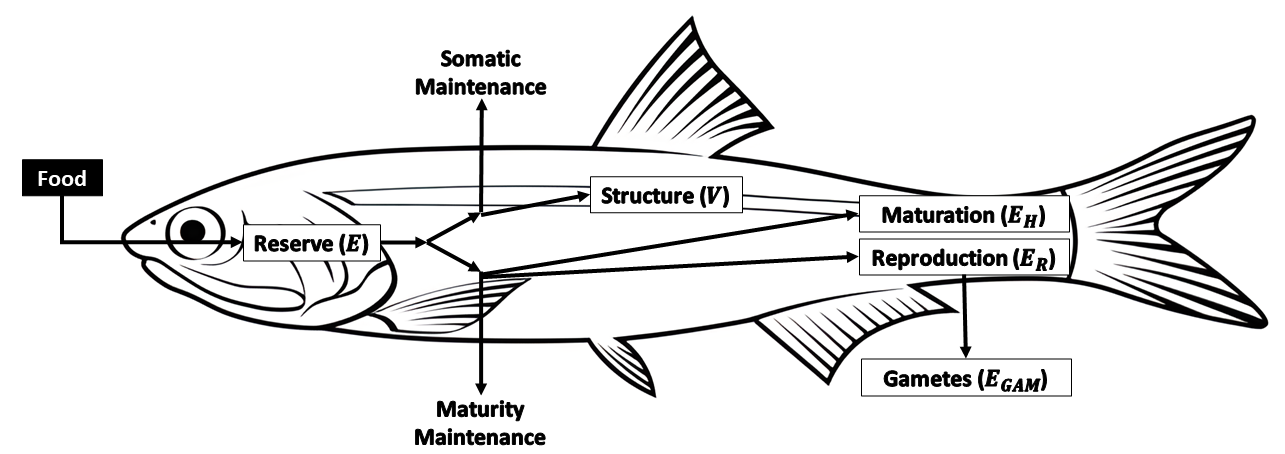
\includegraphics[width=1.0\textwidth]{figures/Chap4_ringens_DEB.png}
	\centering
	\caption{DEB model for E. ringens presented in a flow diagram.}
	\label{Chap4_ringens_DEB}
\end{figure}

\section{Results}

The parameters of the DEB model for Peruvian anchovy (\gls{ringens}) were successfully used to reproduce the larval growth patterns (Fig. \ref{Chap4DEB_out_f1_vsArturoLab}) reported by \citep{RiouOfel2021,OfelMoya2023} assuming a functional response in which food is not a constraint ($f=1$).\\

\begin{figure}[H]
	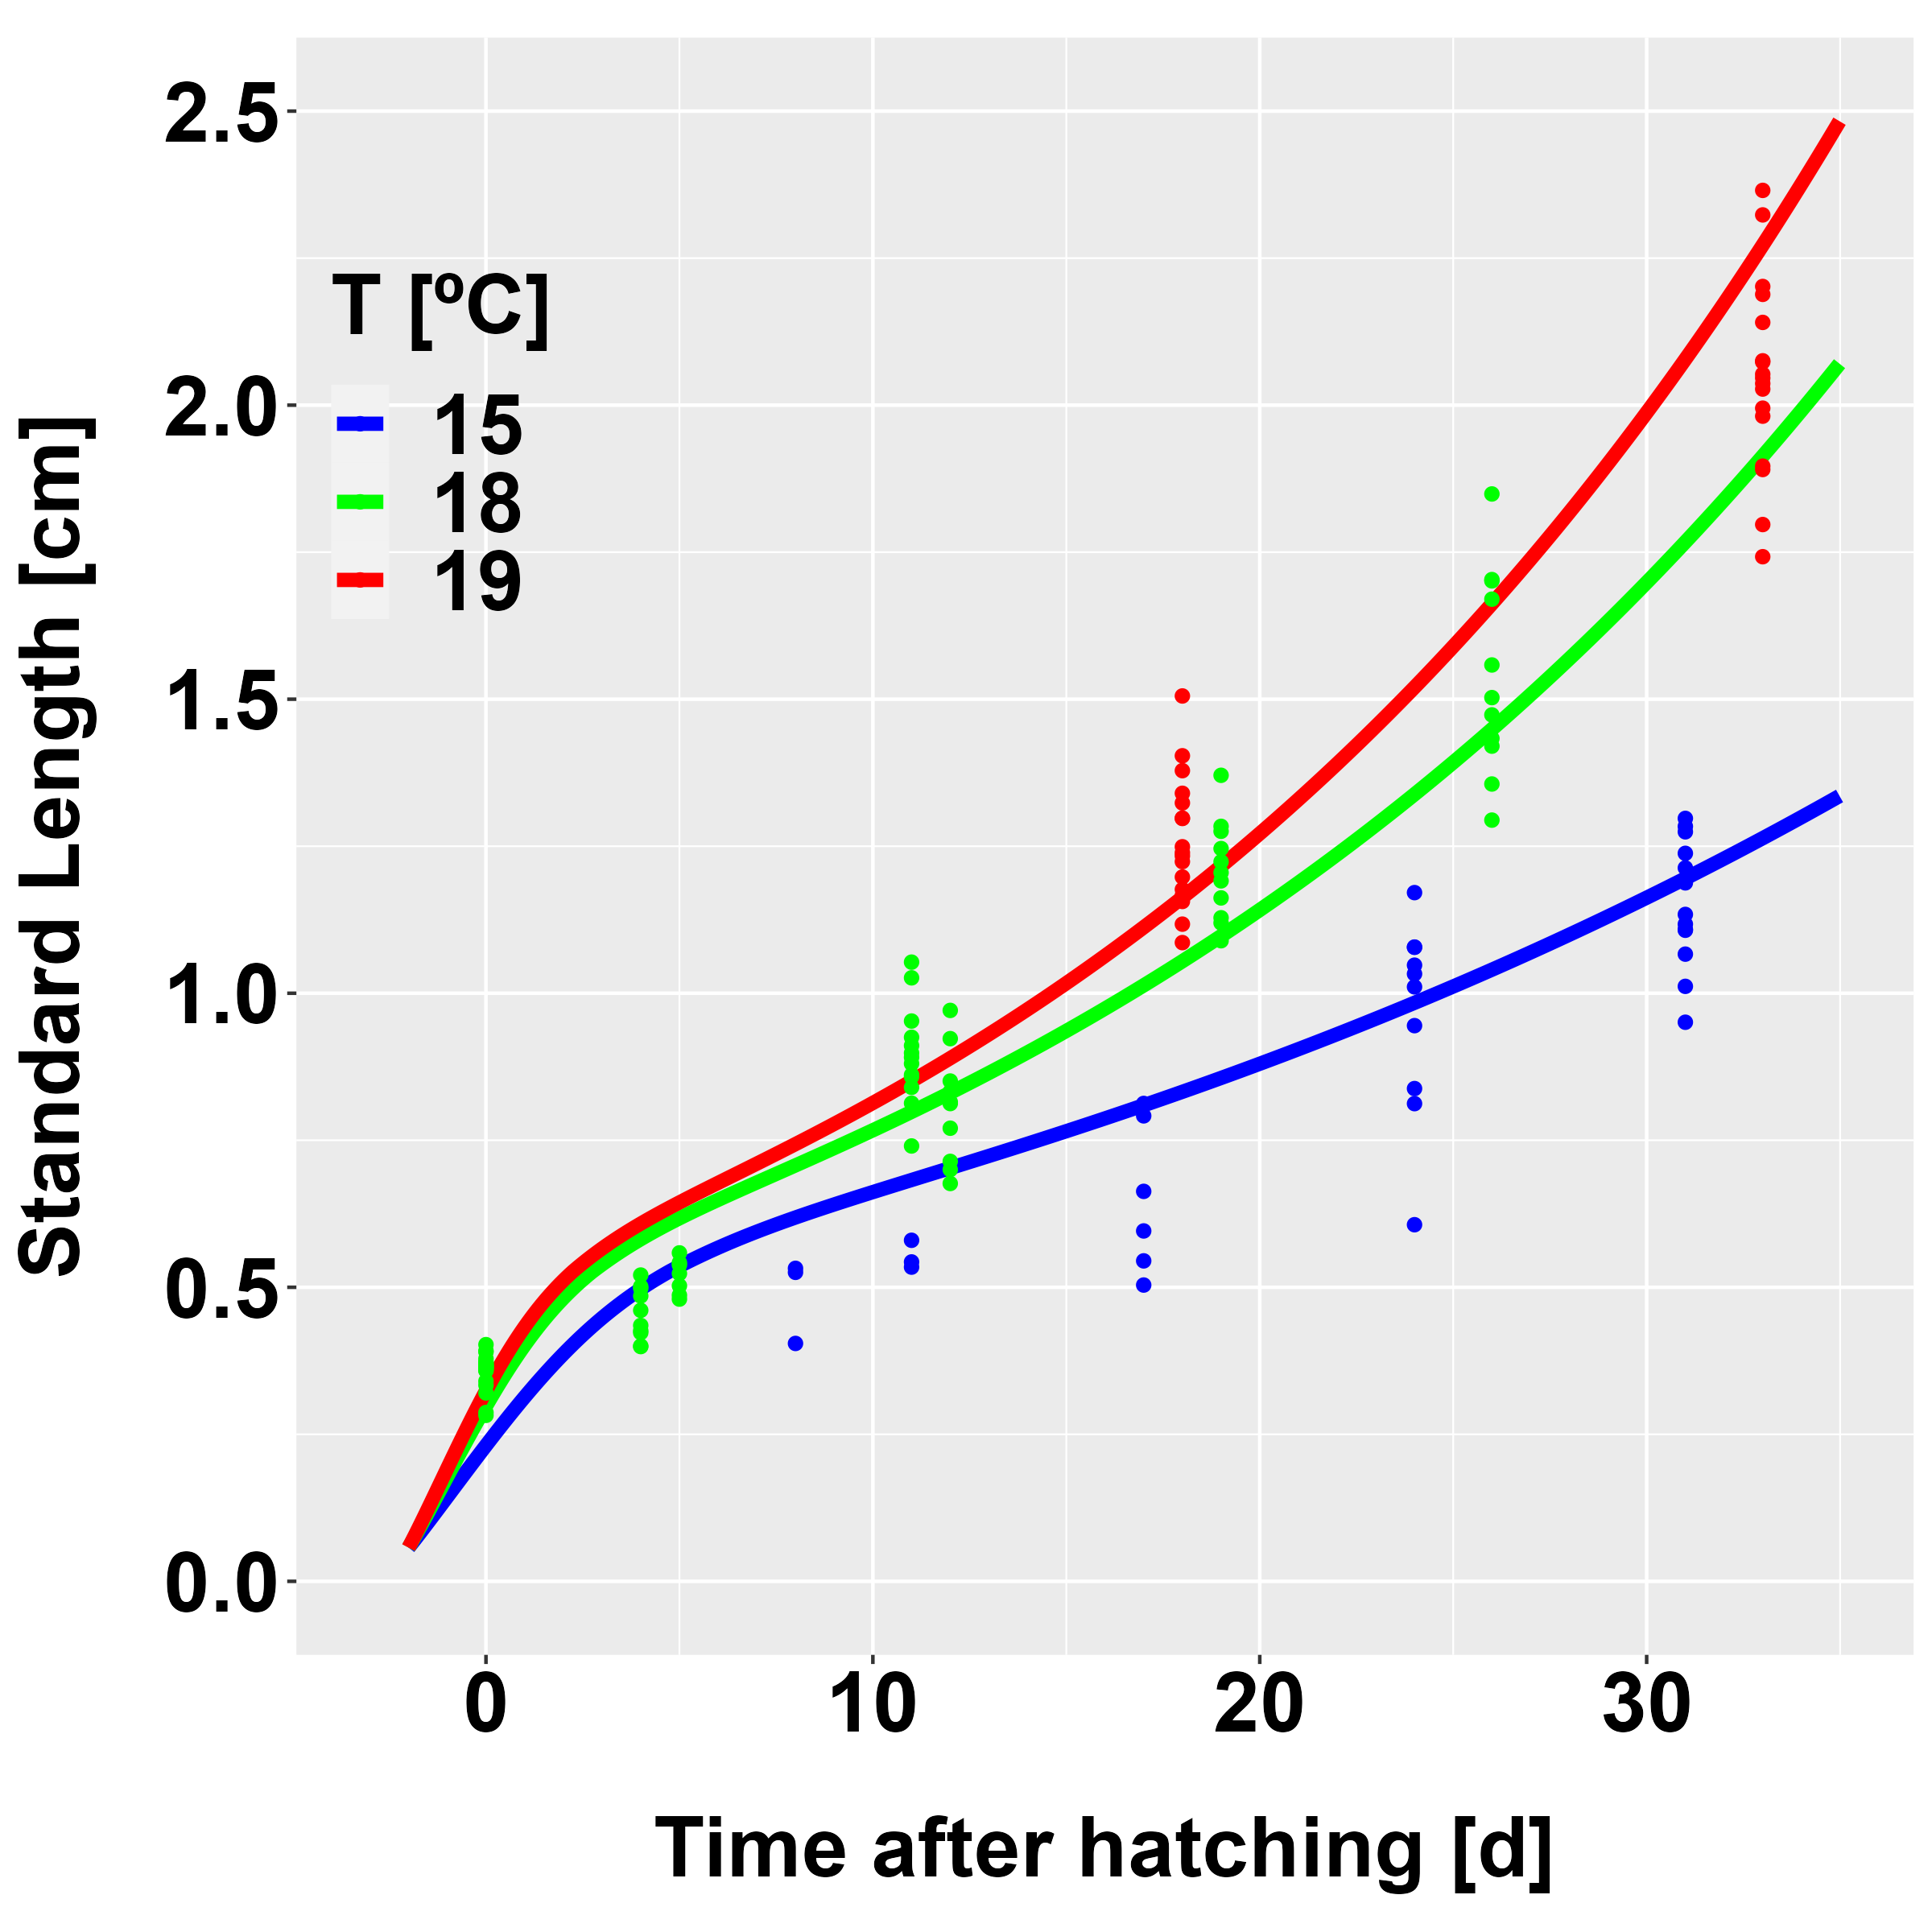
\includegraphics[width=1.0\textwidth]{figures/Chap4DEB_out_f1_vsArturoLab.png}
	\centering
	\caption{Comparison of Peruvian anchovy simulated larval growth (lines) and laboratory observations (dots) from \cite{RiouOfel2021,OfelMoya2023}. The bioenergetic model was calibrated using the data points shown in the graph.}
	\label{Chap4DEB_out_f1_vsArturoLab}
\end{figure}

%\begin{figure}[H]
%	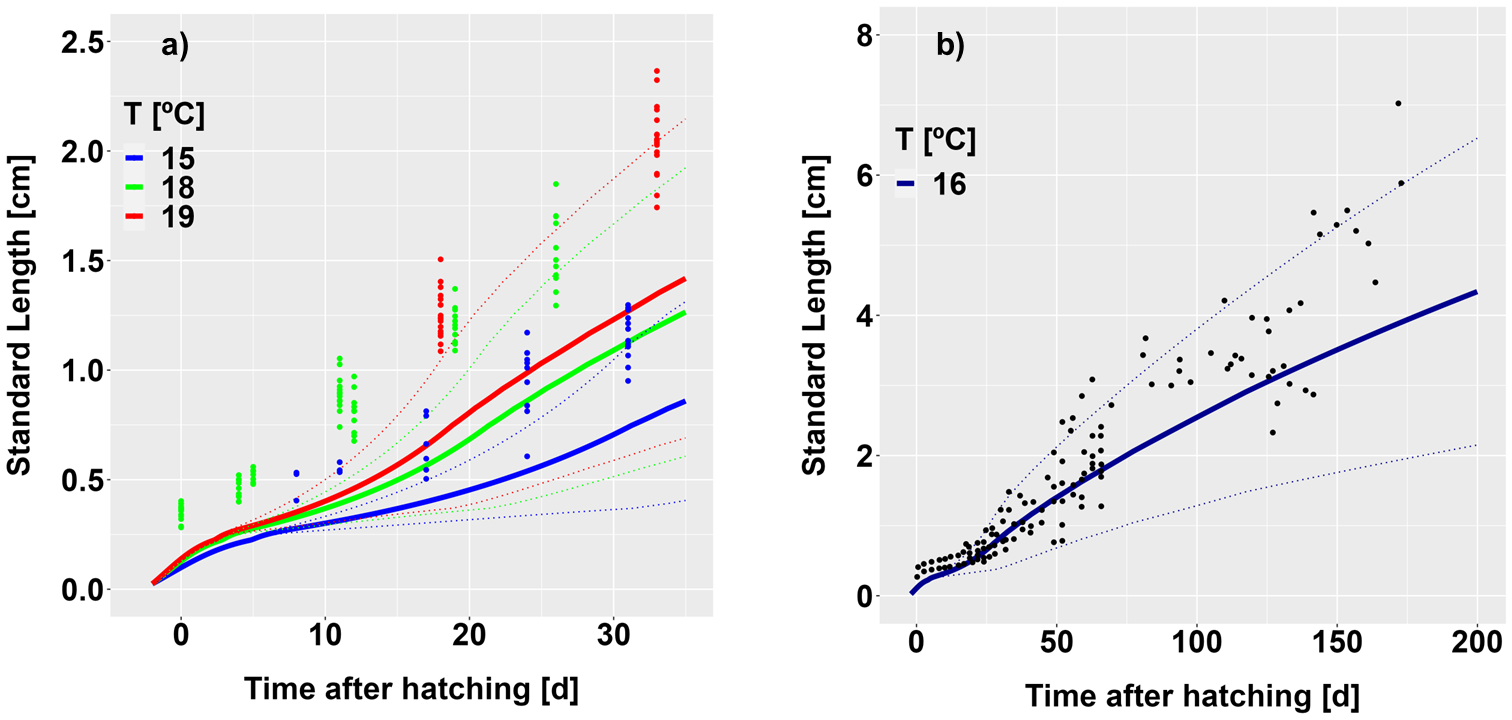
\includegraphics[width=1.0\textwidth]{figures/Chap4DEBvsData.png}
%	\centering
%	\caption{Comparison of Peruvian anchovy simulated larval growth and laboratory observations from \cite{RiouOfel2021} (a) and in situ observations from \cite{MoreClar2011} (b). Thick lines correspond to average size predictions considering ten $f$ values from 0.1 to 1 with 0.1 steps (food limitation factor, see section 2.1.6) at $19$\textdegree $C$ (red), $18$\textdegree $C$ (green) and $15$\textdegree $C$ (blue) in (a) and at $16$\textdegree C in (b). Dotted lines correspond to standard deviation of the simulated larval growth. Colored dots show the corresponding observations. The bioenergetic model was calibrated using the data points shown in the graph. Note that the scales are different in the two panels.}
%	\label{Chap4DEBvsData}
%\end{figure}

In addition, in Fig. \ref{Chap4DEB_out_fMaxMin_vsMoreno2011_larva} we compared the average growth curves resulting from predictions considering ten $f$ values from 0.1 to 1 with 0.1 steps (food limitation factor) versus growth records during their larval stage in individuals reported in \cite{MoreClar2011}, this is because in the natural environment, it is not possible to determine an exact value of the functional response ($f$). It can also be observed that it is possible to reproduce the growth pattern after the larval stage (Fig. \ref{Chap4DEB_out_f1vsMoreno2011_adulto}).\\

\begin{figure}[H]
	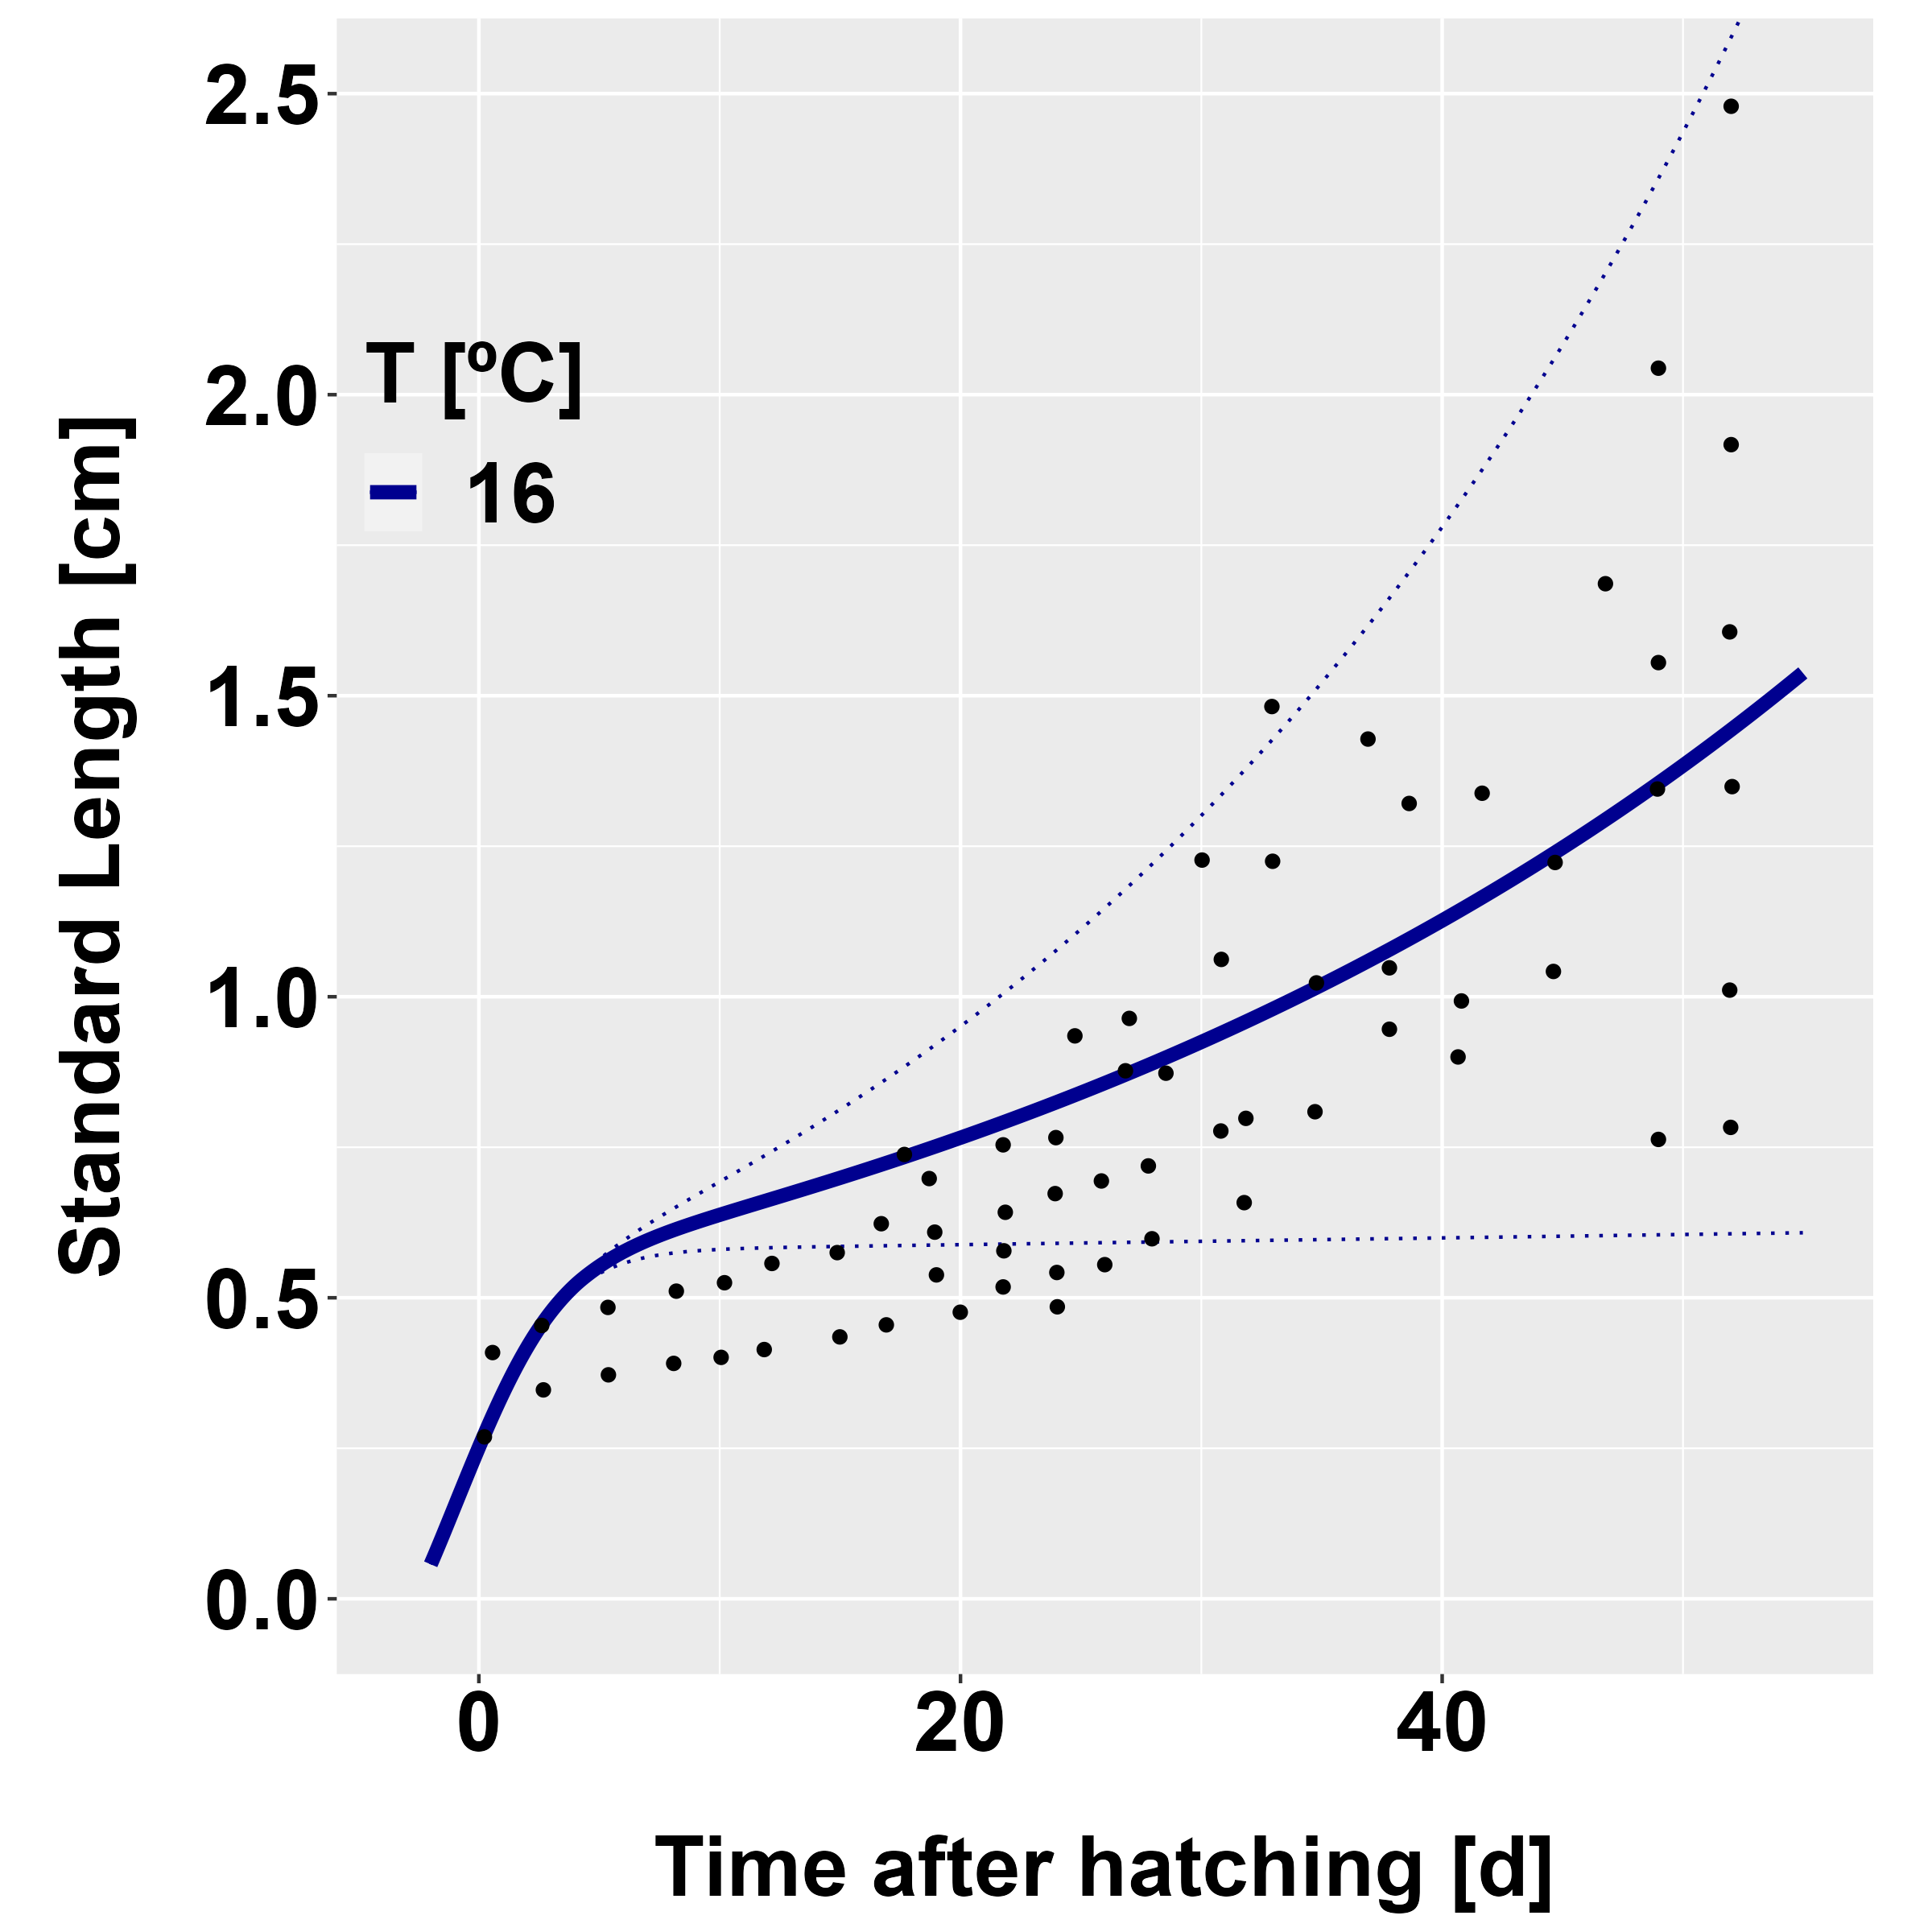
\includegraphics[width=1.0\textwidth]{figures/Chap4DEB_out_fMaxMin_vsMoreno2011_larva.png}
	\centering
	\caption{Comparison of Peruvian anchovy simulated larval growth (blue line) and observations (black dots) from \cite{MoreClar2011}. Dotted lines show the maximum ($f = 1$) and minimum ($f=0.1$)predicted growth obtained with the DEB model.}
	\label{Chap4DEB_out_fMaxMin_vsMoreno2011_larva}
\end{figure}

\begin{figure}[H]
	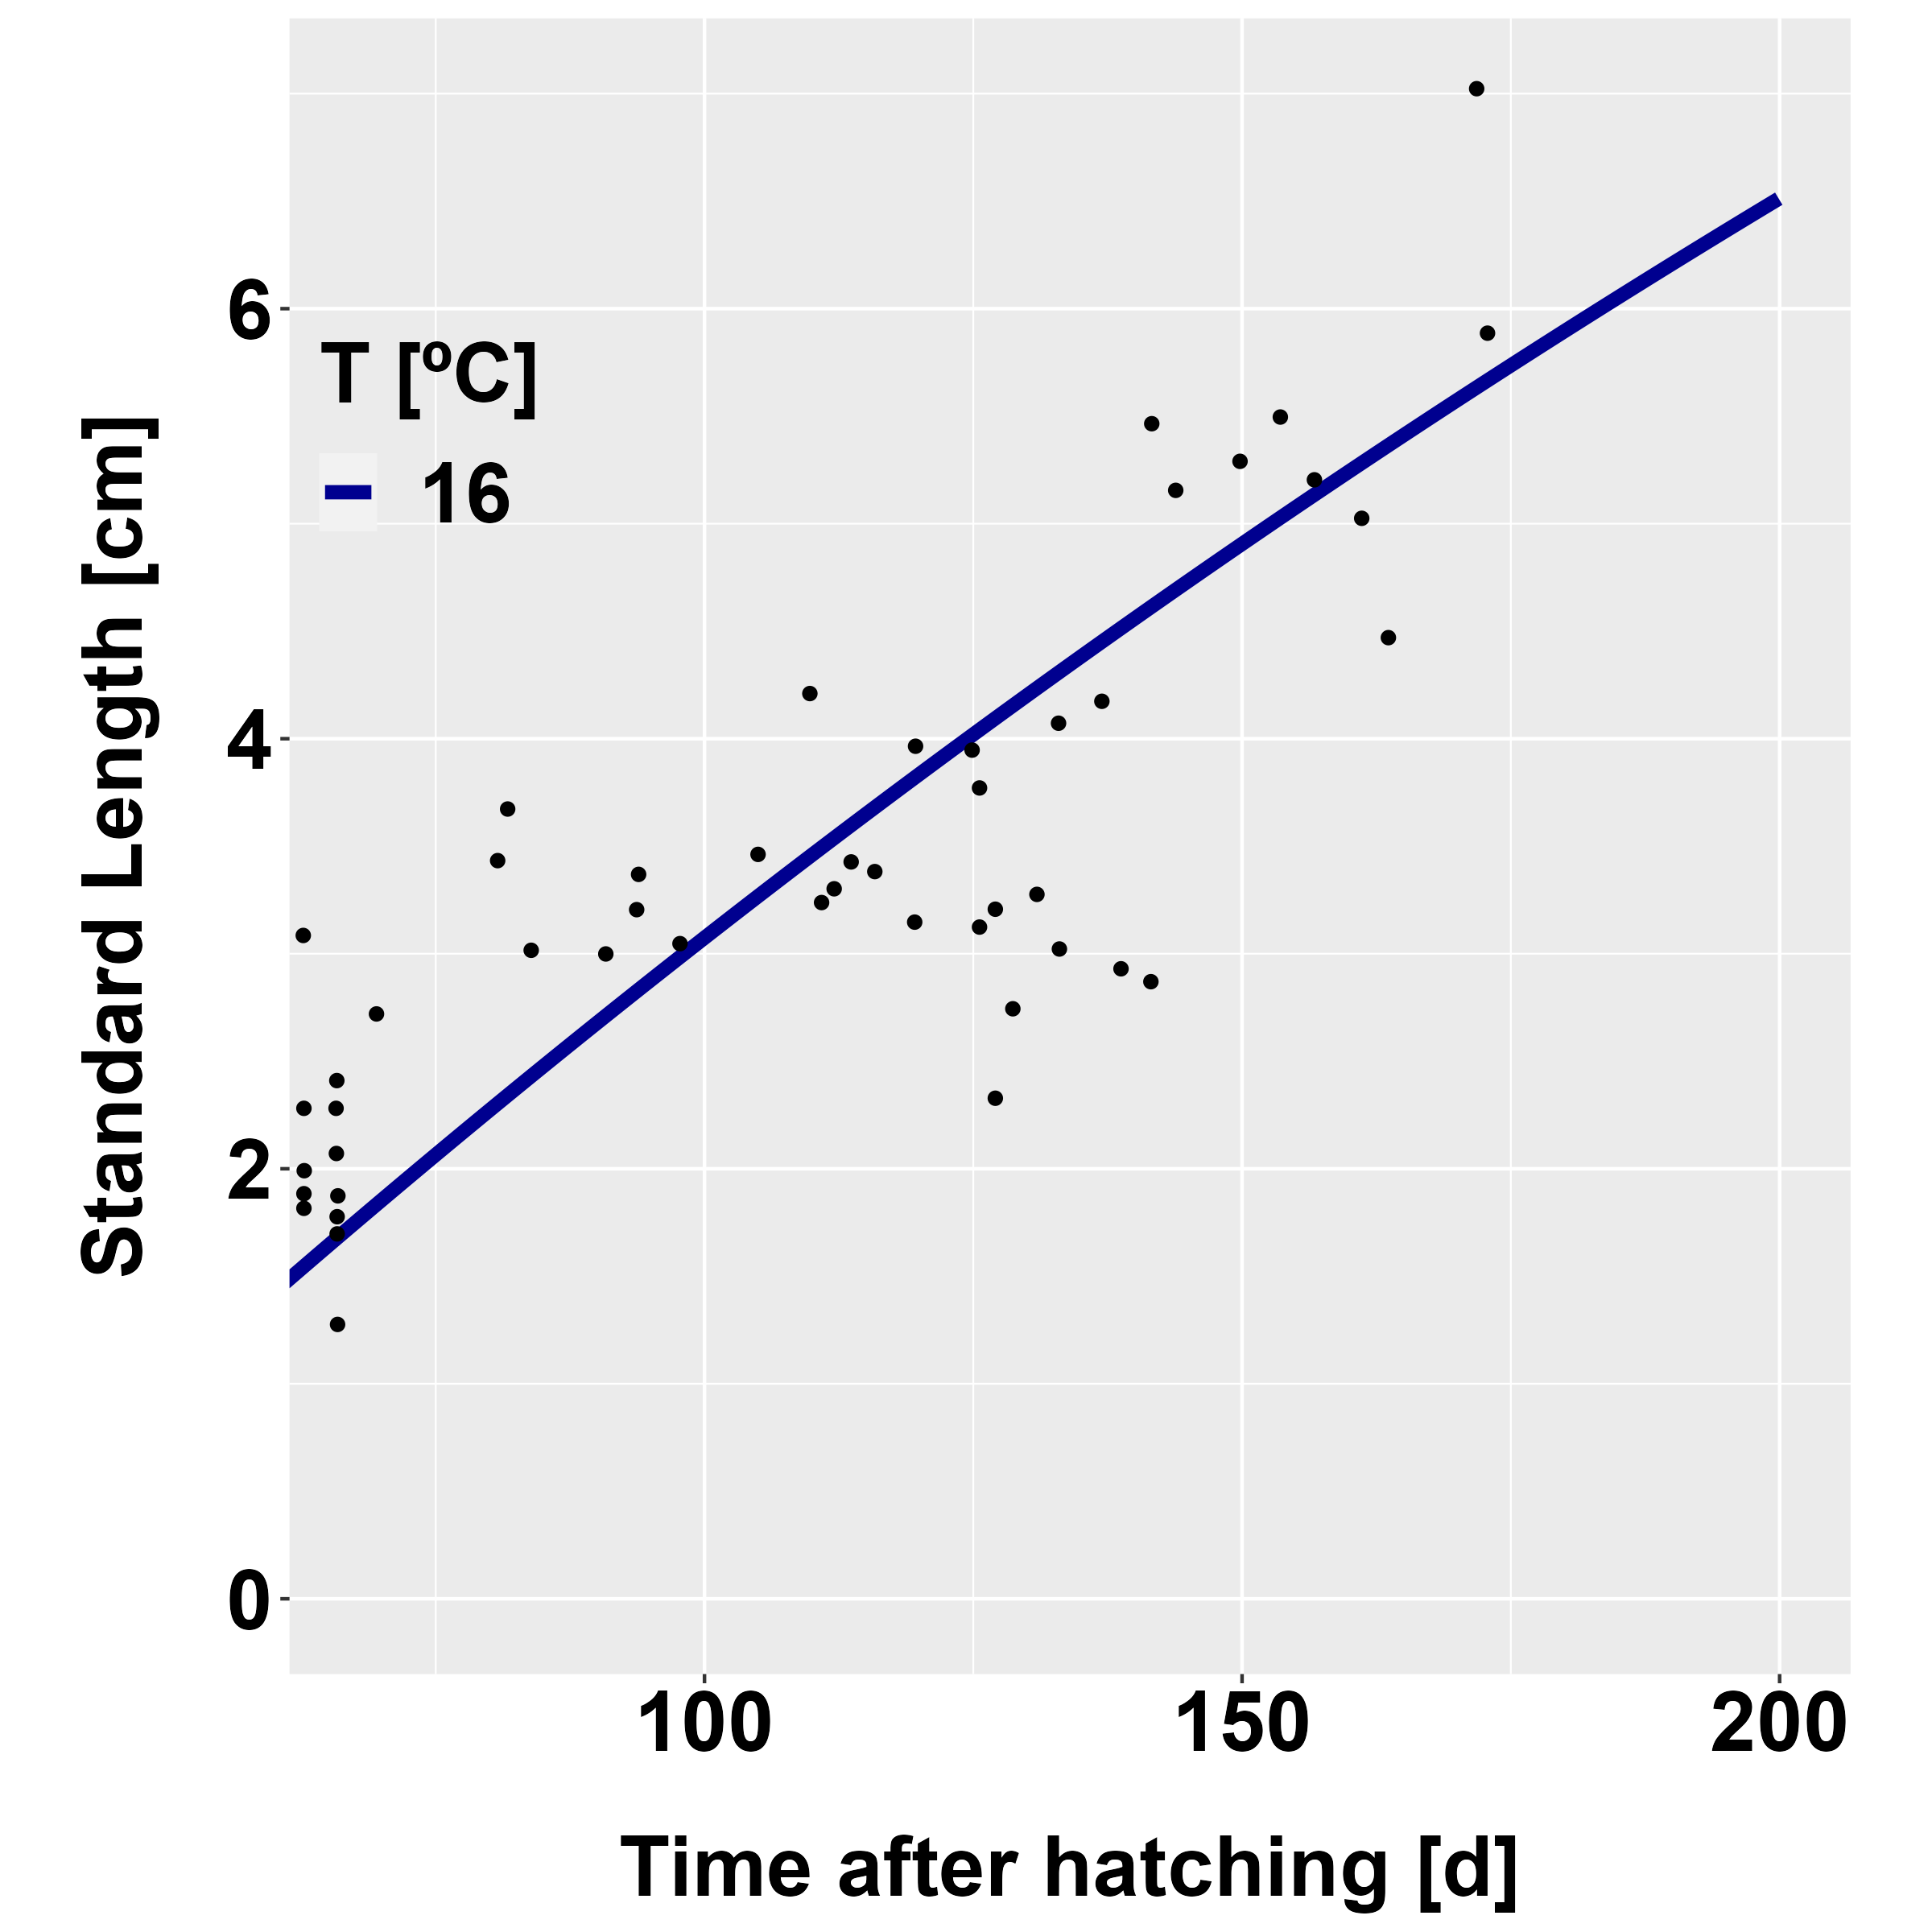
\includegraphics[width=1.0\textwidth]{figures/Chap4DEB_out_f1vsMoreno2011_adulto.png}
	\centering
	\caption{Same as Fig. \ref{Chap4DEB_out_fMaxMin_vsMoreno2011_larva}, but for post larval stage.}
	\label{Chap4DEB_out_f1vsMoreno2011_adulto}
\end{figure}

Starvation tests were conducted on larvae of varying sizes (0.5 and $3 cm$) to investigate the impact of food deprivation on larval recruitment in future simulations. In non-fed conditions, an increase in temperature leads to a starvation effect in fewer days. Furthermore, the \textit{\gls{encrasicolus}} is less sensitive to lack of food than the \gls{ringens}.\\

\begin{figure}[H]
	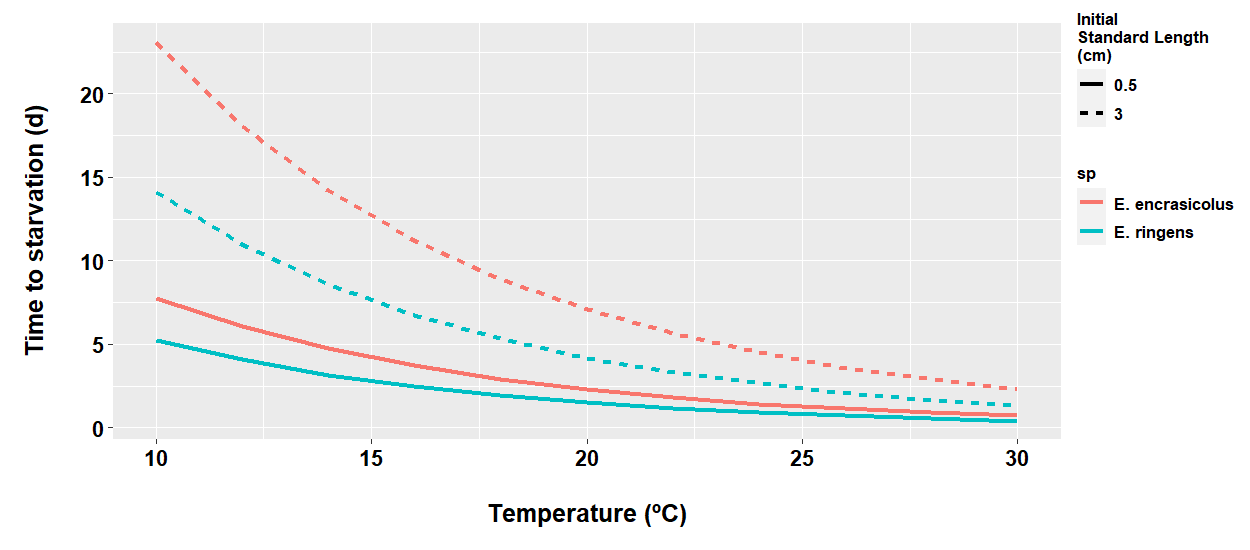
\includegraphics[width=1.0\textwidth]{figures/Chap4Starvation_compar.png}
	\centering
	\caption{Starvation experiments were conducted using the two \acrshort{deb} growth models for \gls{ringens} (green) and \gls{encrasicolus} (orange) larvae of varying sizes ($0.5 cm$ and $3 cm$) at different temperatures, with $f = 0$.}
	\label{Chap4Starvation_compar}
\end{figure}
%\clearpage
%\section{Introduction}\label{Chap4Intro}
%

%
%This theory is particularly popular in ecophysiology and population ecology, where it helps scientists understand how organisms allocate their energy and resources to various life processes, such as growth, maintenance, and reproduction. The DEB theory is based on a set of mathematical equations and concepts that describe how an organism acquires, uses, and allocates energy. These equations take into account factors like energy acquisition (feeding), energy storage, and the trade-offs between various life processes inside the individual. Different individuals (species), present differences that are captured by the DEB theory at the level of their parameter values \citep{Meer2006}. In this way, this theory helps us to understand how a species can flourish or decline, how it competes for resources or how it adapts in different environmental conditions.\\
%
%The strategy is to start from mechanistic considerations at the individual level incorporating details about the physiology of the species defining parameters that describe how the organism acquires, allocates, and uses energy \citep{KooiSabe1986}. These parameters include assimilation rates, growth rates, reproduction rates, maintenance costs, and more, all of which are typically influenced by factors like temperature, food availability, and age, cementing the basic blocks to model studies on \textit{Engraulis ringens} structured population.\\
%
%\textit{E. ringens}, commonly known as the Peruvian anchovy, is a small pelagic fish species found in the southeastern Pacific Ocean along the coasts of South America, particularly in the Humboldt Current system \citep{GutiSwar2007}. Along with the Peruvian anchovy, there is usually an important presence of sardine (\textit{Sardinops sagax}), another small pelagic species, but since the decade of the 2000s, there have been no significant landings off the peruvian coast \citep{CardFran2015}, and the fact that \textit{E. ringens} is usually associated with the coastal zone while sardines occupy more oceanic areas due to different feeding and oxygen conditions \citep{EspiBert2008,BertChai2011}, we can study the interaction of anchovy with their environment without considering a competition with sardines.\\
%
%When commercially targeted marine fish feed on phytoplankton and zooplankton, they assimilate and redistribute essential nutrients, influencing the productivity and structure of the ecosystem \citep{LeMeGuie2022}. Also, anchovies help maintain the balance and stability of marine ecosystems due their population dynamics can impact the abundance of other species, influencing ecosystem health and resilience to environmental changes \citep{FennSear2023}. Since Dynamic Energy Budget theory can be used in IBM models, ecosystem models, toxicology models \citep{LavaFilg2021}, a DEB model for \textit{E. ringens} is essential for future ecological studies and for conservation purposes.
%
%Below, we list some important concepts in DEB modelling:
%
%\begin{itemize}
%%  \centering
%  \item Energy Budget: DEB modeling starts by quantifying the energy fluxes into and out of an organism. This includes energy gained through feeding, losses due to metabolism and maintenance, growth, reproduction, and other processes.\\
%  
%  \item Allocation and Utilization: The model describes how the acquired energy is allocated and utilized for different biological processes, such as growth, reproduction, and maintenance. It helps to understand how organisms prioritize energy allocation under varying conditions.\\
%
%  \item Reserves and Structure: DEB models account for the storage of surplus energy as reserves (e.g., fat, proteins) and the development of structural components (e.g., organs, tissues). The dynamics of these reserves are critical in understanding an organism's life history.\\
%
%  \item Maintenance and Maturation: DEB models consider the energy spent on maintaining basic bodily functions (maintenance) and the energy used for growth and development (maturation) at different life stages.\\
%
%  \item Environmental Factors: The model incorporates two principal environmental factors like temperature, food availability, and other abiotic factors (not taken into account in this study) to assess their influence on energy acquisition, utilization, and allocation.\\
%
%\end{itemize}
%
%In addition, we present a list of potential uses of a DEB model:
%
%\begin{itemize}
%%  \centering
%  \item Growth and Development: DEB models provide insights into the growth patterns and development stages of organisms. They help predict how growth rates vary with environmental conditions and resource availability.\\
%  
%  \item Reproduction and Life History Strategies: DEB models enable the study of reproductive strategies, including the timing and allocation of energy to reproduction. This aids in understanding reproductive trade-offs and strategies for optimizing its survival.\\
%  
%  \item 	Responses to Environmental Change: DEB models help predict how organisms respond to changes in environmental conditions, such as temperature, nutrient availability, and pollution. This is crucial for assessing the impacts of climate change and other environmental stressors.\\
%  
%  \item Optimizing Fisheries and Aquaculture: DEB models aid in optimizing fisheries and aquaculture practices by predicting growth rates, maturation, and reproduction, leading to sustainable management of fish stocks.\\
%  
%  \item Toxicology and Ecotoxicology: Although it is not the objective of this study, DEB models can be applied to assess the effects of toxins and pollutants on an organism's energy allocation and life history traits, aiding in understanding toxicological impacts.\\
%
%\end{itemize}
%
%So, in this chapter, we will start by showing the available data collection, the calibration of a DEB model with growth acceleration during its early life stages (that was not taken into account in the Chapter \ref{Chap3}) and its implementation in the IBM called Ichthyop-DEB model, to explore the interaction of the species with its environment, focusing mainly on its food demand since the effect of temperature has been well documented previously.
%
%\section{Methods}\label{Chap4Meth}
%
%\subsection{Data collection}\label{Chap4MethDat}
%
%A model is composed of mathematical equations that represent the characteristics of a dynamic system. These equations include parameters that allow the comparison of different systems, and these parameters are estimated from empirical data \citep{RaolGiri2004}. Gather empirical data and literature data related to \textit{E. ringens}, includes growth rates, especially in their early stages of life, reproduction rates, feeding rates, body sizes, and any other relevant biological measurements.\\
%
%In spite of the application of DEB theory is challenging because the state variables and parameters are abstract quantities that are not directly observable, the parameter estimation method \citep{Lika2011a,Lika2011b} makes use of different data sources.\\
%
%However, there are different levels of difficulty in collecting individual or population data for a species. For example, a collection of population data for \textit{E. ringens} is well described by \citep{MarzShin2009}, but data on metabolic rates, feeding rates or vertical behaviour (characteristics that require captive breeding) have been studied more in other similar species and other ecosystems \citep{AldaCota2008,CermUria2003,KramZwei1968,DetwHoud1970,Hunt1971,Hunt1984,SakaKimu1976,Houd1977,MethKram1979,Thei1980,Brow1983}, while laboratory rearing (especially for early life stages) is just beginning for \textit{E. ringens} \citep{RiouOfel2021,OfelMoya2023}, difficulty in rearing, which can be explained by the high migratory behaviour of anchovies in general \citep{OlivSala2001,MoraBaba2010,TanaOhsh2010,PoliHure2015,GuraFach2017,CastNiqu2021}.\\
%
%The following is a description of the available and preferably most updated data used for DEB parameters estimation on \textit{E. ringens}.\\
%
%\subsection{Parameter estimation}
%
%Estimating parameters for a Dynamic Energy Budget (DEB) model involves a process to fit the model to empirical data, allowing it to accurately represent the energy allocation and life history of a specific organism, in this case, \textit{E. ringens}.\\
%
%We used a bivariate statistical technique \citep{Lika2011a,Lika2011b} to estimate the values of the model parameters that minimize the difference between model predictions and observed data. Then, we fitted the DEB model to the compiled empirical data, adjusting parameters to best represent the biological processes and energy dynamics of \textit{E. ringens}.\\
%
%In order to show the difference between the DEB-standard model (\textit{E. encracicolus}) used in Chapter \ref{Chap3}, a comparative table with the estimated parameters for \textit{E. ringens} is presented below.
%
%Table 1: Parameters used for the bioenergetic model describing larval growth. These values were estimated by Pethybridge et al. (2013) for Engraulis encrasicolus and compared with the parameters estimated for E. ringens (current study). The values of $T_L$, $T_H$, $T_AL$, $T_AH$ are detailed for case 1. Values for case 2 are indicated in parenthesis when different from case 1.

